\chapter{User Manual}
\thispagestyle{fancy}

To quickly have a look at what was realized during the semester thesis, just 
install the \textit{Toggle Function Definition} code automation according to 
this manual.

\section{Installation of the Plug-in}

To try out the plug-in, you will need a running Eclipse Helios (3.6) installation with CDT already installed. Choose "Help", "Install New Software..." and type in the following url into the address bar:

\url{http://sinv-56042.edu.hsr.ch/updatesite}

The plug-in may now be installed using the install wizard. Be aware that the 
update site is hosted on a virtual server that will be removed at the end of 
summer 2011. However, a copy of the whole virtual server may be found on the 
attached CD.

\subsection{Activate the Menu Item}

\begin{figure}[h]
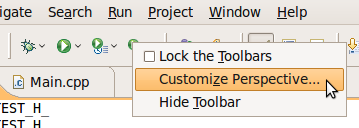
\includegraphics[width=0.4\textwidth]{images/customizeperspective.png}
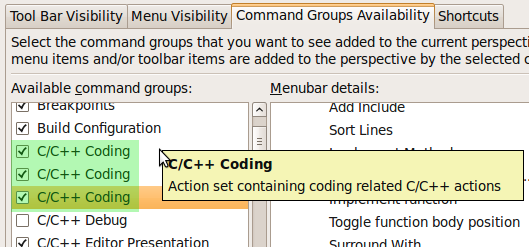
\includegraphics[width=0.6\textwidth]{images/commandgroups.png}
\caption{To use the refactoring from the menu, it needs to be enabled manually 
after installation.}
\label{showMenu}
\end{figure}
\label{cmdGroup}
To run the refactoring using the menu, some changes have to be applied to the 
current perspective. Right-click on the toolbar and choose 
"Customize perspective...". Then go to the "Groups and commands visibility" tab 
and check \textbf{all} "C++ coding" boxes. The menu "Toggle Function Definition" 
should now be visible inside the source menu.

\section{Using the Refactoring}

Toggling is available whenever the cursor is inside a function declaration 
or definition. Any selection between the first and the last character of 
the function definition (without comments) is considered valid for toggling. 
Figure \ref{selection} depicts all valid selection ranges in an example code.
\begin{figure}[h]
\centering
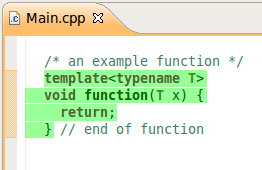
\includegraphics[width=0.4\textwidth]{images/selection.png}
\caption{region for valid selection positions}
\label{selection}
\end{figure}
As soon as the cursor is inside the valid range, toggling may be invoked by 
pressing \texttt{Ctrl+Alt+v}.

\section{Example}

\begin{figure}[h]
\centering
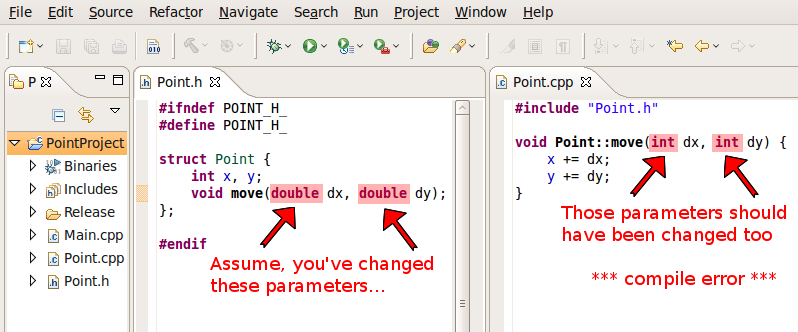
\includegraphics[width=\textwidth]{images/differing_signatures.png}
\caption{redundant declarations that were not both updated}
\label{differingSignatures}
\end{figure}
Imagine the situation in figure \ref{differingSignatures} where a programmer 
forgot to update a function signature of a function that was defined inside 
another file.
After finding and correcting the signatures, the programmer would like to define 
the function directly inside the header file, removing the redundancy of a 
separate definition. What would he do?

Perhaps he would jump to the definition, copy its body, remove the definition, 
jump back to the declaration, remove its semicolon, add curly brackets and paste 
the copied function body. All in all, seven actions.

\subsection{The Solution}
This is the point where \textit{Toggle Function Body} makes life easier. Imagine 
the same situation (with correct signatures though) and the user presses the key 
combination \texttt{ctrl+shift+V}. Figure \ref{coolResult} shows what happens to 
the code. The declaration got automatically replaced by the definition.

\begin{figure}[h]
\centering
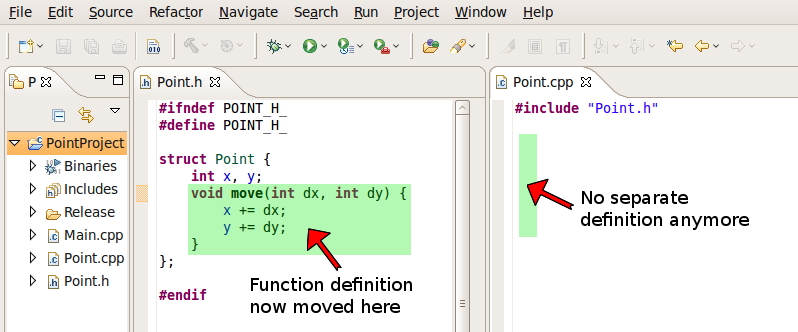
\includegraphics[width=\textwidth]{images/resulting_function.png}
\caption{by the touch of a key combination, the function definition is moved}
\label{coolResult}
\end{figure}

The function is now defined in one place and its signature may be changed 
without updating the declaration separately. Seven actions have been replaced by 
just one keystroke. Convinced?

